\chapter{Resultados}
\label{cap:resultados}

Este capítulo presenta los resultados del trabajo. La evaluación se ha realizado en un
entorno de simulación que reproduce la pila de software completa del robot y permite
ejercitar el sistema de extremo a extremo. Sobre ese entorno se aporta una doble
evidencia: una \textbf{validación funcional}, que comprueba que el ciclo operativo
completo se ejecuta de principio a fin, y un primer conjunto de \textbf{métricas
cuantitativas} de cartografía, navegación, detección y rendimiento. La réplica de esta
evaluación sobre el robot físico, una vez disponible el hardware, se delimita de forma
explícita como trabajo pendiente en la Sección~\ref{sec:pruebas-real}.

%% =============================================================================
\section{Entorno y escenario de pruebas}
\label{sec:entorno-pruebas}

La evaluación se ha llevado a cabo en simulación, sobre el modelo del \mbox{TurtleBot~4}
ejecutado en \textit{Gazebo}, con \textit{RViz} como herramienta de visualización del
estado del robot, los sensores y el mapa. El mundo simulado es un entorno interior de tipo
laberinto, con varios corredores y bifurcaciones, que ejercita la navegación a través de
pasillos estrechos y giros. Este entorno integra la misma pila de software que se
ejecutaría sobre el robot físico (\gls{ros} Humble, \gls{nav2}, \texttt{slam\_toolbox} y
\texttt{explore\_lite}), de modo que los nodos propios del proyecto y el backend operan sin
cambios respecto al despliegue real. Esta equivalencia permite ejercitar la lógica completa
del sistema (la máquina de estados del orquestador, la generación de la ruta, la detección
y los flujos de datos) sin depender todavía del hardware.

\begin{notebox}{Pendiente de la campaña sobre hardware real}
  La descripción del escenario físico definitivo (dimensiones de la estancia, disposición
  de los obstáculos y condiciones de iluminación) se incorporará tras la ejecución de las
  pruebas sobre el robot real, planteadas en la Sección~\ref{sec:pruebas-real}.
\end{notebox}

%% =============================================================================
\section{Validación funcional}
\label{sec:validacion-funcional}

En primer lugar, la validación se ha orientado a verificar la correcta integración de los
subsistemas y la coherencia de los flujos de datos entre el robot, el bus de eventos, el
backend y la aplicación de usuario. Sobre el entorno de simulación se ha ejercitado el
ciclo operativo completo, comprobando que cada flujo descrito en el
Capítulo~\ref{cap:desarrollo} se ejecuta de principio a fin y produce el efecto esperado en
los almacenes de datos y en la interfaz.

En particular, se ha confirmado que el robot explora el entorno y construye su mapa, que la
\gls{fsm} encadena de forma autónoma las fases del ciclo (exploración, guardado,
planificación y patrulla), que la ruta de cobertura se deriva del mapa y se recorre de forma
cíclica, y que la detección de una persona dispara el registro de una incidencia con su
vídeo asociado. Asimismo, se ha verificado que la telemetría llega a InfluxDB y se visualiza
en Grafana, y que las órdenes emitidas desde la aplicación (iniciar, detener y reinstalar la
patrulla) se propagan hasta el robot y se reflejan en su estado. La
tabla~\ref{tab:validacion} resume estas comprobaciones.

\begin{table}[htbp]
  \centering
  \small
  \caption{Resumen de la validación funcional realizada en simulación. Fuente:
  elaboración propia.}
  \label{tab:validacion}
  \begin{tabular}{@{}>{\raggedright\arraybackslash}p{4.3cm}
                     >{\raggedright\arraybackslash}p{6.2cm}
                     >{\raggedright\arraybackslash}p{2.7cm}@{}}
    \toprule
    \textbf{Flujo o prueba} & \textbf{Cobertura} & \textbf{Resultado} \\
    \midrule
    Autenticación del robot & \gls{tofu}, autenticación y refresco del \gls{jwt} &
    Verificado (sim.) \\
    \addlinespace[3pt]
    Exploración y mapeo & \texttt{explore\_lite} y \texttt{slam\_toolbox} &
    Verificado (sim.) \\
    \addlinespace[3pt]
    Guardado del mapa & Servicio \texttt{map\_saver} &
    Verificado (sim.) \\
    \addlinespace[3pt]
    Generación de la ruta & Barrido en zig-zag sobre el mapa &
    Verificado (sim.) \\
    \addlinespace[3pt]
    Patrulla cíclica & Recorrido de \textit{waypoints} con \gls{nav2} &
    Verificado (sim.) \\
    \addlinespace[3pt]
    Acople y desacople & Acciones \texttt{dock}/\texttt{undock} del Create~3 &
    Verificado (sim.) \\
    \addlinespace[3pt]
    Localización sobre mapa guardado & \texttt{map\_server} y AMCL (modo localización) &
    Verificado (sim.) \\
    \addlinespace[3pt]
    Detección de incidencia & \gls{yolo} $\rightarrow$ MinIO $\rightarrow$ Kafka
    $\rightarrow$ registro & Verificado (sim.) \\
    \addlinespace[3pt]
    Telemetría & \texttt{serve\_telemetry} $\rightarrow$ InfluxDB $\rightarrow$ Grafana &
    Verificado (sim.) \\
    \addlinespace[3pt]
    Control desde la aplicación & Iniciar, detener y reinstalar la patrulla &
    Verificado (sim.) \\
    \addlinespace[3pt]
    Estado operativo & \textit{Heartbeat} $\rightarrow$ PostgreSQL $\rightarrow$ app &
    Verificado (sim.) \\
    \bottomrule
  \end{tabular}
\end{table}

Estas comprobaciones confirman que la arquitectura es coherente y que los subsistemas se
integran según el diseño. A partir de ellas, las secciones siguientes cuantifican el
comportamiento del sistema en simulación.

%% =============================================================================
\section{Resultados de simulación}
\label{sec:resultados-sim}

Más allá de la validación funcional, sobre el mismo entorno de simulación se ha recogido un
primer conjunto de métricas cuantitativas, organizadas según las dimensiones definidas en
la Sección~\ref{sec:metricas}: cartografía y navegación, detección de incidencias y
rendimiento de extremo a extremo.

% ---------------------------------------------------------------------------
\subsection{Cartografía y ruta de patrulla}
\label{sec:resultados-cartografia}

El robot explora el entorno de forma autónoma con \texttt{explore\_lite} mientras
\texttt{slam\_toolbox} construye el mapa de ocupación (figura~\ref{fig:mapa-slam}). A partir
de ese mapa, el orquestador deriva la ruta de cobertura en zig-zag y la recorre de forma
cíclica; la figura~\ref{fig:ruta-patrulla} muestra la trayectoria seguida sobre el mapa ya
consolidado.

\begin{figure}[H]
  \centering
  \begin{subfigure}[t]{0.48\textwidth}
    \centering
    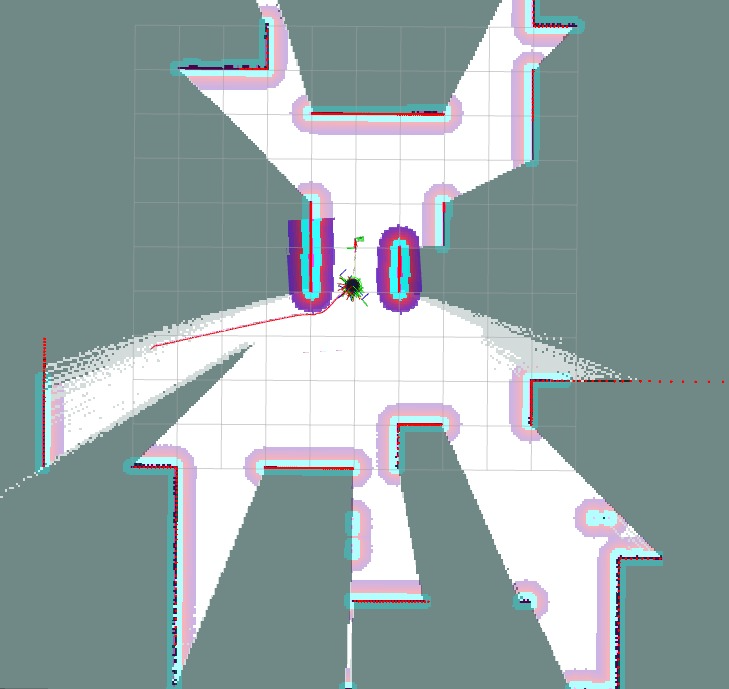
\includegraphics[width=\linewidth, alt={Mapa de ocupación construido por SLAM durante la exploración, visualizado en RViz}]{recursos/figuras/resultados/mapa-slam.png}
    \caption{Mapa construido por SLAM.}
    \label{fig:mapa-slam}
  \end{subfigure}
  \hfill
  \begin{subfigure}[t]{0.48\textwidth}
    \centering
    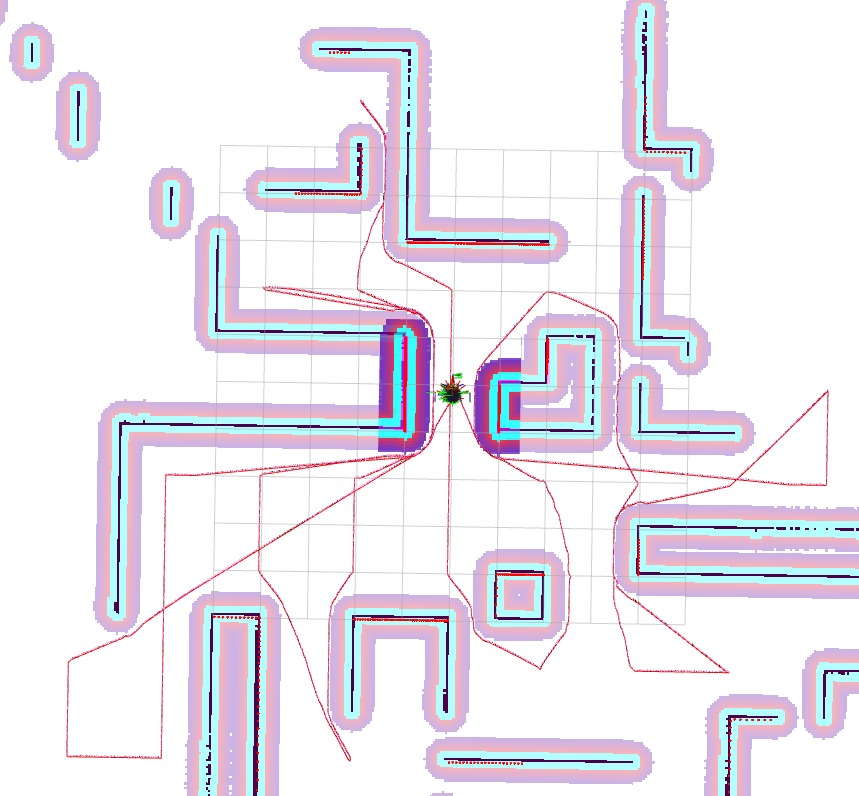
\includegraphics[width=\linewidth, alt={Ruta de patrulla recorrida por el robot sobre el mapa, visualizada en RViz}]{recursos/figuras/resultados/ruta-patrulla.png}
    \caption{Ruta de patrulla sobre el mapa.}
    \label{fig:ruta-patrulla}
  \end{subfigure}
  \caption[Mapa y ruta de patrulla en simulación]{Cartografía y patrulla en simulación
    (RViz): (a)~mapa de ocupación construido por \texttt{slam\_toolbox} durante la
    exploración (blanco: espacio libre; rosa y morado: paredes y su inflado; gris: sin
    explorar); (b)~trayectoria de la patrulla (en rojo) sobre el mapa consolidado, derivada
    del barrido en zig-zag del espacio libre. Fuente: elaboración propia.}
  \label{fig:mapa-ruta}
\end{figure}

El mapa resultante, guardado con resolución de 0,05\,m por celda, cubre un lienzo de
$390\times401$ celdas (unos $19{,}5\times20{,}1$\,m). De la región ya explorada, en torno al
96{,}5\,\% de las celdas corresponde a espacio libre y el 3{,}5\,\% restante a paredes, lo
que arroja un área libre navegable de aproximadamente $185{,}5$\,m\textsuperscript{2}. La
tabla~\ref{tab:metricas-navegacion} recoge estas magnitudes junto con las métricas de
navegación que completan la corrida de patrulla.

\begin{table}[htbp]
  \centering
  \small
  \caption{Métricas de cartografía y navegación en simulación. Fuente: elaboración propia.}
  \label{tab:metricas-navegacion}
  \begin{tabular}{@{}>{\raggedright\arraybackslash}p{7.5cm} l l@{}}
    \toprule
    \textbf{Métrica} & \textbf{Unidad} & \textbf{Valor} \\
    \midrule
    Resolución del mapa                      & m/celda & 0,05 \\
    Extensión cartografiada (lienzo)         & m       & 19,5 $\times$ 20,1 \\
    Área libre navegable                     & m\textsuperscript{2} & $\approx$185,5 \\
    Paredes sobre la región explorada        & \%      & 3,5 \\
    Tiempo de exploración del mapa           & s       & 840 \\
    Waypoints generados en la ruta           & nº      & 29  \\
    Waypoints alcanzados sin intervención    & \%      & 29  \\
    Comportamientos de recuperación de Nav2  & nº      & 2   \\
    Colisiones durante la patrulla           & nº      & 0   \\
    Tiempo por ciclo de patrulla             & s       & 1200\\
    \bottomrule
  \end{tabular}
\end{table}

\begin{notebox}{Inciso sobre la obtención de métricas en simulación}
  Las métricas de la tabla~\ref{tab:metricas-navegacion} de carácter temporal resultan afectadas por 
la velocidad de simulación, que depende de la carga de la máquina y de la complejidad del
mundo virtual.
\end{notebox}

% ---------------------------------------------------------------------------
\subsection{Detección de incidencias}
\label{sec:resultados-deteccion}

La capacidad de detección se evalúa sobre un escenario controlado en simulación, con 162
apariciones en posiciones e instantes conocidos durante la patrulla: 120 de personas y 42 de
objetos que no lo son, entre ellos un maniquí de apariencia humana como caso deliberadamente
ambiguo. El nodo \texttt{detect\_incident} aplica el modelo YOLOv8n a cada fotograma y, al
superar el umbral de confianza, dispara la incidencia. La figura~\ref{fig:deteccion-sim}
ilustra una detección durante la simulación. Comparando las apariciones reales con las
detecciones se obtienen los verdaderos y falsos positivos y los falsos negativos, y de ellos
la precisión y el \textit{recall}; la tabla~\ref{tab:metricas-deteccion} recoge estos valores
junto con la confianza media y el tiempo de inferencia.

\begin{figure}[H]
  \centering
  \IfFileExists{recursos/figuras/resultados/deteccion-sim.png}
    {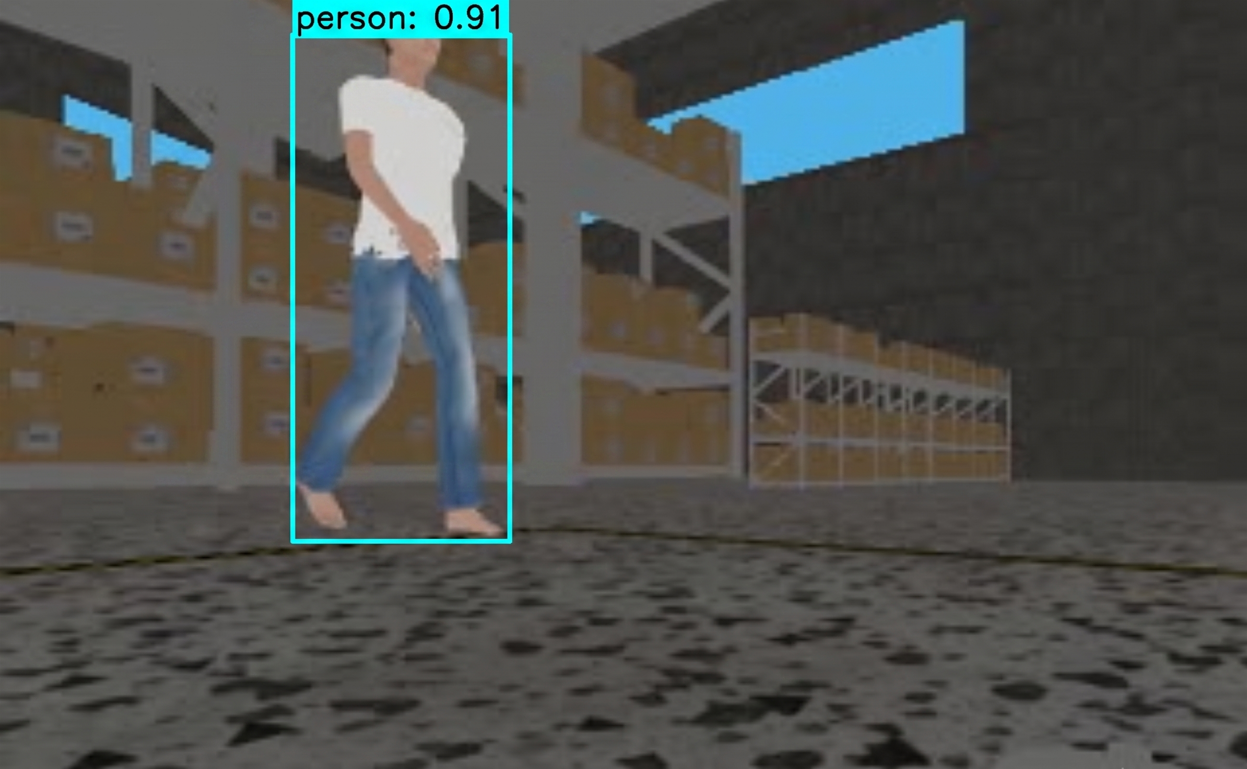
\includegraphics[width=0.72\textwidth, alt={El robot detecta a una persona en la simulación}]{recursos/figuras/resultados/deteccion-sim.png}}
    {\fbox{\parbox[c][5cm][c]{0.72\textwidth}{\centering\itshape Captura de la detección de
      una persona en simulación (pendiente de incorporar en
      \texttt{recursos/figuras/resultados/deteccion-sim.png}).}}}
  \caption[Detección de una persona en simulación]{Detección de una persona durante la
    patrulla en simulación, que dispara el registro de la incidencia. Fuente: elaboración
    propia.}
  \label{fig:deteccion-sim}
\end{figure}

\begin{table}[htbp]
  \centering
  \small
  \caption{Métricas de detección sobre el escenario controlado en simulación. Fuente:
  elaboración propia.}
  \label{tab:metricas-deteccion}
  \begin{tabular}{@{}>{\raggedright\arraybackslash}p{7.5cm} l l@{}}
    \toprule
    \textbf{Métrica} & \textbf{Unidad} & \textbf{Valor} \\
    \midrule
    Apariciones evaluadas                     & nº     & 162 \\
    \quad de persona (positivos reales)       & nº     & 120 \\
    \quad de no-persona (negativos reales)    & nº     & 42 \\
    Verdaderos positivos                      & nº     & 120 \\
    Falsos negativos                          & nº     & 0 \\
    Falsos positivos                          & nº     & 7 \\
    Verdaderos negativos                      & nº     & 35 \\
    Precisión                                 & [0, 1] & 0,945 \\
    \textit{Recall}                           & [0, 1] & 1,000 \\
    Confianza media de detección              & [0, 1] & 0,899 \\
    Tiempo de inferencia                      & ms/fotograma & 80,3 \\
    \bottomrule
  \end{tabular}
\end{table}

El detector se enfrentó a 162 apariciones controladas durante la patrulla, de las cuales 120
correspondían a personas y 42 a objetos de otra naturaleza. Sobre las 120 apariciones de
persona el modelo acertó en todas, sin un solo falso negativo, y lo hizo con una confianza
media de 0,899, lo que indica detecciones no solo correctas sino también firmes. El
\textit{recall} resultante es, por tanto, perfecto (1,000).

Frente a las 42 apariciones que no eran personas, el modelo las descartó correctamente en 35
ocasiones y se equivocó en 7, todas ellas sobre un maniquí de apariencia humana, el caso más
exigente del conjunto. Esos siete falsos positivos son la única fuente de error y rebajan la
precisión a 0,945, un valor todavía elevado y coherente con un sistema cuya prioridad es no
pasar por alto a ninguna persona. El tiempo medio de inferencia fue de 80,3\,ms por fotograma;
conviene precisar que se midió sobre la \acrshort{cpu} del equipo de simulación y no sobre el
hardware del robot, por lo que constituye una referencia en ese entorno y no el rendimiento
esperable a bordo.

% ---------------------------------------------------------------------------
\subsection{Validación del flujo de extremo a extremo}
\label{sec:resultados-e2e}

Por último, se valida el flujo completo de notificación de principio a fin. En simulación se ha
comprobado que una incidencia detectada por el robot recorre toda la cadena sin intervención
manual: el nodo \texttt{detect\_incident} publica el evento en Kafka, el consumidor del backend
lo registra como un \texttt{Incidente} en PostgreSQL y la aplicación lo lista y reproduce el
clip almacenado en MinIO. De forma análoga, la telemetría que el robot publica una vez por
segundo llega a InfluxDB y se visualiza en Grafana (figura~\ref{fig:grafana}), y el
\textit{heartbeat} de estado, emitido cada diez segundos, actualiza el estado operativo que la
aplicación refleja en la pantalla de inicio. El sistema funciona, por tanto, de extremo a
extremo en simulación.

La latencia absoluta percibida, desde que la persona aparece hasta que la incidencia es visible
en la aplicación, no se reporta en este entorno: el simulador opera por debajo del tiempo real y
el clip incorpora además un tramo de fotogramas posteriores grabados a la cadencia reducida de
la cámara simulada, de modo que cualquier medida en reloj de pared resultaría inflada y no
representativa. Su caracterización se reserva para la campaña sobre hardware real
(sección~\ref{sec:pruebas-real}). Sí se recogen, en cambio, las magnitudes cuyo valor no depende
del factor de tiempo real de la simulación, por ejecutarse en el anfitrión o por referirse a la
fiabilidad del flujo, que la tabla~\ref{tab:metricas-e2e} resume.

\begin{table}[htbp]
  \centering
  \small
  \caption{Métricas del flujo de extremo a extremo medibles en simulación, independientes del
  factor de tiempo real. Fuente: elaboración propia.}
  \label{tab:metricas-e2e}
  \begin{tabular}{@{}>{\raggedright\arraybackslash}p{7.5cm} l l@{}}
    \toprule
    \textbf{Métrica} & \textbf{Unidad} & \textbf{Valor} \\
    \midrule
    Telemetría recibida frente a la esperada (1\,Hz nominal)      & \% & 100 \\
    Latencia evento en Kafka $\rightarrow$ registro en PostgreSQL & ms & 503 \\
    Tiempo de subida del clip a MinIO (media de 20 incidencias)   & s  & 3,7 \\
    \bottomrule
  \end{tabular}
\end{table}

Las magnitudes recogidas confirman la solidez del flujo en el lado del servidor, cuyo rendimiento
no depende de la velocidad de la simulación. La telemetría se recibió sin pérdidas, con todos los
puntos esperados a la cadencia nominal de un punto por segundo. La subida de cada clip de
incidencia a MinIO tardó 3,7\,s de media sobre veinte incidencias, un tiempo dominado por la
escritura y la transferencia del vídeo. Por último, la latencia desde la llegada del evento a
Kafka hasta su registro en PostgreSQL fue de 503\,ms; este valor está dominado por el ciclo de
sondeo del consumidor, que espera los mensajes en intervalos de hasta un segundo
(\texttt{poll(1.0)}), más que por el procesamiento o la escritura en la base de datos, y podría
reducirse acortando ese intervalo.

%% =============================================================================
\section{Pruebas en el robot real}
\label{sec:pruebas-real}

Toda la evaluación anterior se ha obtenido en simulación. Su réplica sobre el
\mbox{TurtleBot~4} físico permitirá contrastar las métricas en condiciones reales, donde
influyen la dinámica del robot, el ruido de los sensores y la iluminación del entorno. Esta
campaña está planificada y pendiente de ejecución.

\begin{notebox}{TODO: campaña de pruebas sobre hardware real}
  Pendiente de realizar sobre el robot físico, replicando la evaluación de simulación:
  \begin{itemize}
    \item Descripción del escenario físico (dimensiones, obstáculos e iluminación).
    \item Métricas de cartografía y navegación (tabla~\ref{tab:metricas-navegacion}) sobre
      el entorno real.
    \item Métricas de detección (tabla~\ref{tab:metricas-deteccion}) con personas reales.
    \item Latencias de extremo a extremo (tabla~\ref{tab:metricas-e2e}) en la red de
      despliegue.
    \item Comparación de los resultados reales con los obtenidos en simulación.
  \end{itemize}
\end{notebox}

%% =============================================================================
\section{Discusión}
\label{sec:discusion}

Los primeros resultados cuantitativos, obtenidos en simulación, junto con la validación
funcional, permiten afirmar que la arquitectura propuesta es coherente y que sus componentes
se integran según el diseño previsto. El desacoplamiento mediante el bus de eventos ha
facilitado el desarrollo y la prueba de cada subsistema por separado: cada flujo se ha podido
ejercitar de forma aislada y, después, en conjunto, sin que la indisponibilidad puntual de un
componente bloqueara a los demás. Este comportamiento respalda la decisión de diseño
adoptada.

No obstante, la validación en simulación tiene límites que conviene reconocer. El entorno
simulado no reproduce con fidelidad la dinámica del robot real, el ruido de los sensores ni
las condiciones de iluminación, factores que inciden directamente tanto en la navegación
como en la percepción. Por ello, las principales incógnitas que la campaña sobre hardware
real deberá despejar son el comportamiento de la navegación en presencia de obstáculos
dinámicos, la fiabilidad del detector en condiciones reales de iluminación y la latencia del
flujo completo de notificación. Estas cuestiones se retoman, junto con las limitaciones del
trabajo, en el Capítulo~\ref{cap:conclusiones}.
